\section{Results}
\label{sec:results}

\section{Results for evolutionary approach 1}
\label{sec:results_1}

Like in section \ref{sec:challenges} already mentioned unstable simulation results and non-reproducibility were encountered which make it hard to interpret the results. Thus, good weights are interpreted mostly as weights with a high potential for a good reward.\\
The same evolutionary algorithm was tested with slightly different configurations concerning hyper-parameters. 
The best distances within every generation were plotted with a logarithmic scale and can be seen in figure \ref{fig:results_1}. 

\begin{figure}[H]
	\centering
	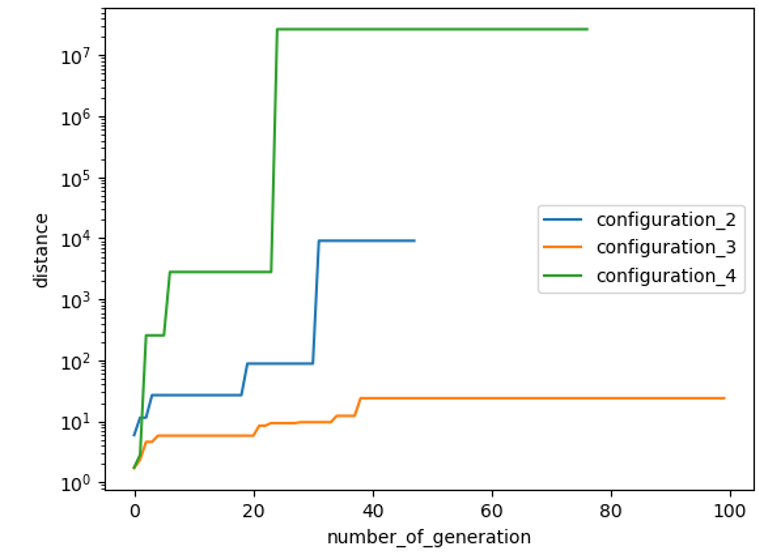
\includegraphics[width=3.3in]{img/results_1.png}
	\DeclareGraphicsExtensions.
	\caption{Results for different experiment configurations}
	\label{fig:results_1}
\end{figure}

The simulations were executed with the following 4 different configurations:\\

\begin{itemize}
\item Configuration 1: 
\begin{itemize}
\item Output: 4 neurons to control 4 joints
\item fix input of value 1
\item result was not plotted, overall best distance: 25 meters
\end{itemize}
\item Configuration 2: 
\begin{itemize}
\item Output: 7 neurons, 7 Joints 
\item Input: Position of Box (x, y, z) coordinates
\end{itemize}
\item Configuration 3: 
\begin{itemize}
\item Output: 7 neurons, 7 Joints 
\item Input: Position of Box rounded to second decimal place
\end{itemize}
\item Configuration 4: 
\begin{itemize}
\item Output: 7 neurons, 7 Joints and scaled output weights 
\item Input: Position of Box rounded to second decimal place
\end{itemize}
\end{itemize}


In general there is to say that our algorithm found weights with high potential for a huge distance in short time and optimized those weights like desired before but a big part of the distances were instabilities of the calculation in the platform. Furthermore the best distances were only sparsely reproducible due to non instability of the simulation but the algorithm still performed well on the given prerequisites. 

\section{Conclusion}

A brief introduction into genetic algorithms, reinforcement learning and spiking neural networks were given and the reason for the algorithm choice of the given task was elaborated. The different approaches were described theoretically and problems were discussed. Finally the results are given for each of the approaches and its sub-configurations and an interpretation of those was given. 